% A '%' character causes TeX to ignore all remaining text on the line,
% and is used for comments like this one.

\documentclass{article}      % Specifies the document class
\usepackage{amsmath, nccmath}
\usepackage{enumitem}
\usepackage{graphicx}
\usepackage[utf8]{inputenc}
\usepackage{listings}
\usepackage{xcolor}
\graphicspath{ {./} }
\definecolor{codegreen}{rgb}{0,0.6,0}
\definecolor{codegray}{rgb}{0.5,0.5,0.5}
\definecolor{codepurple}{rgb}{0.58,0,0.82}
\definecolor{backcolour}{rgb}{0.95,0.95,0.92}
\usepackage{float}
\lstdefinestyle{mystyle}{
    backgroundcolor=\color{backcolour},   
    commentstyle=\color{codegreen},
    keywordstyle=\color{magenta},
    numberstyle=\tiny\color{codegray},
    stringstyle=\color{codepurple},
    basicstyle=\ttfamily\footnotesize,
    breakatwhitespace=false,         
    breaklines=true,                 
    captionpos=b,                    
    keepspaces=true,                 
    numbers=left,                    
    numbersep=5pt,                  
    showspaces=false,                
    showstringspaces=false,
    showtabs=false,                  
    tabsize=2
}

\lstset{style=mystyle}

\title{CEE 498 Applied Machine Learning - HW5}  % Declares the document's title.
\author{Rini Jasmine Gladstone (rjg7) and Maksymillian Podraza(podraza3)}      % Declares the author's name.
\date{April 13, 2020}      % Deleting this command produces today's date.

\newcommand{\ip}[2]{(#1, #2)}
                             % Defines \ip{arg1}{arg2} to mean
                             % (arg1, arg2).

%\newcommand{\ip}[2]{\langle #1 | #2\rangle}
                             % This is an alternative definition of
                             % \ip that is commented out.

\begin{document}             % End of preamble and beginning of text.

\maketitle                   % Produces the title.


\section{Problem 1}      % Produces section heading.  Lower-level
                             % sections are begun with similar 
                             % \subsection and \subsubsection commands.

\subsection{Part a}

We used the following image for our analysis.

\begin{figure}[H]
\centering
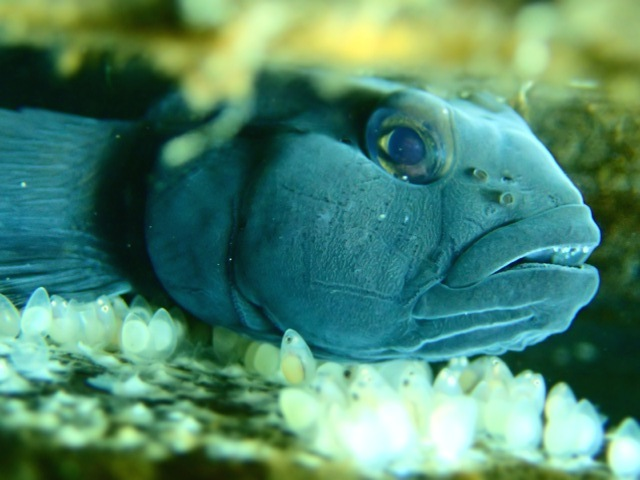
\includegraphics[width=0.7\textwidth]{RobertMixed03.jpg}
\end{figure}

We normalized the image so that the darkest pixel takes the value (0,0,0) and the lightest pixel takes the value (1,1,1).

\begin{lstlisting}
image_paths = ["RobertMixed03.jpg", "smallstrelitzia.jpg", "smallsunset.jpg"]

def load_images():
    image_array = []
    try:
        for image_path in image_paths:
            img = Image.open(image_path)
            image_array.append(img)
    except IOError: 
        pass
    return image_array

images = load_images()

working_image = images[0]

def image_matrix_create(image):
    image_matrix = []
    img_w, img_h = image.size
    image_data = list(image.getdata())
    for y in range(img_h):
        image_matrix.append(image_data[y*img_w:(y+1)*img_w])
    image_df = pd.DataFrame(image_matrix)
    return image_df

def rgb_extract(image):
    rgb = []
    for i in range(3):
        rgb.append(image.apply(lambda x: [y[i] for y in x]))
    return rgb

def rgb_normalize(image):
    normalized = []
    for i in range(3):
        x = image[i].values 
        min_max_scaler = preprocessing.MinMaxScaler()
        x_scaled = min_max_scaler.fit_transform(x)
        df = pd.DataFrame(x_scaled)
        normalized.append(df)
    return normalized

r = image_matrix_create(working_image)
rgb_matrix_list = rgb_extract(r)
rgb_normalized_list = rgb_normalize(rgb_matrix_list)
\end{lstlisting}

Then, we wrote the function for EM.
\begin{lstlisting}
def EM_function(X,cov,k,niter):    
        weights = np.ones((k)) / k
        means = np.random.choice(X.values.flatten(), (k,X.shape[1]))
        eps=1e-8
        likelihood = []
        log_likelihoods = []
        for step in range(niter):
            likelihood = []
            # Expectation step
            for j in range(k):
                likelihood.append(multivariate_normal.pdf(x=X, mean=means[j], cov=cov[j],allow_singular=True))
            likelihood = np.array(likelihood)
            assert likelihood.shape == (k, len(X))
            b = []
            # Maximization step 
            for j in range(k):
                # use the current values for the parameters to evaluate the posterior
                # probabilities of the data have been generated by each gaussian
                b.append((likelihood[j] * weights[j]) / (np.sum([likelihood[i] * weights[i] for i in range(k)], axis=0)+eps))
                # update mean and variance
                means[j] = np.sum(b[j].reshape(len(X),1) * X, axis=0) / (np.sum(b[j]+eps))
                cov[j] = np.dot((b[j].reshape(len(X),1) * (X - means[j])).T, (X - means[j])) / (np.sum(b[j])+eps)
                # update the weights
                weights[j] = np.mean(b[j])
                assert cov.shape == (k, X.shape[1], X.shape[1])
                assert means.shape == (k, X.shape[1])
            log_likelihoods.append(np.log(np.sum([k*multivariate_normal(means[i],cov[j],allow_singular=True).pdf(X) for k,i,j in zip(weights,range(len(means)),range(len(cov)))])))
            if (step+1)%100==0 and (step+1)>=100:
                print(step+1)
        return means,cov,weights,b,log_likelihoods,likelihood
\end{lstlisting}

We set the initial covariance matrix (cov) to be identity matrix and ran the following code setting k = 10, 20 and 50.

\begin{lstlisting}
rvalues=rgb_normalized_list[0].values.flatten()
gvalues=rgb_normalized_list[1].values.flatten()
bvalues=rgb_normalized_list[2].values.flatten()
list_of_tuples = list(zip(rvalues, gvalues, bvalues))  
data=pd.DataFrame(list_of_tuples, columns = ['R', 'G', 'B'])
#Number of clusters
k=50
#Initializing the covariance matrix
cov = []
for i in range(k):
    cov.append(np.eye(data.shape[1]))
cov = np.array(cov)
means,cov,weights,b,log_likelihoods,likelihood=EM_function(data,cov,k,1000)
#Plotting the log-likelihood
plt.plot(log_likelihoods)
likelihood = np.array(likelihood)
#Finding the closest cluster for each pixel
predictions = np.argmax(likelihood, axis=0)
data['cluster']=predictions
data['mean_R']=np.zeros(data.shape[0])
data['mean_G']=np.zeros(data.shape[0])
data['mean_B']=np.zeros(data.shape[0])
for i in range(data.shape[0]):
    data.at[i,'mean_R']=means[data.at[i,'cluster']][0]
    data.at[i,'mean_G']=means[data.at[i,'cluster']][1]
    data.at[i,'mean_B']=means[data.at[i,'cluster']][2]
for i in range(k):
    data['weight_c'+str(i)]=b[i]
\end{lstlisting}

We ran the code for 1000 iterations. The convergence of log likelhood values for 10 clusters is as shown below. 

\begin{figure}[H]
\centering
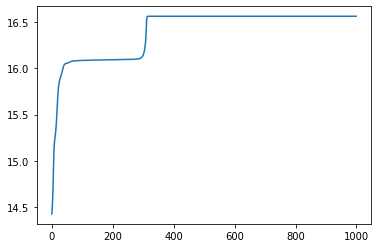
\includegraphics[width=0.7\textwidth]{Convergence_parta_10}
\end{figure}

The values converge around 400 iterations.

The following are the images obtained by replacing each pixel with the mean of its cluster center.     

   
\begin{figure}[H]
\centering
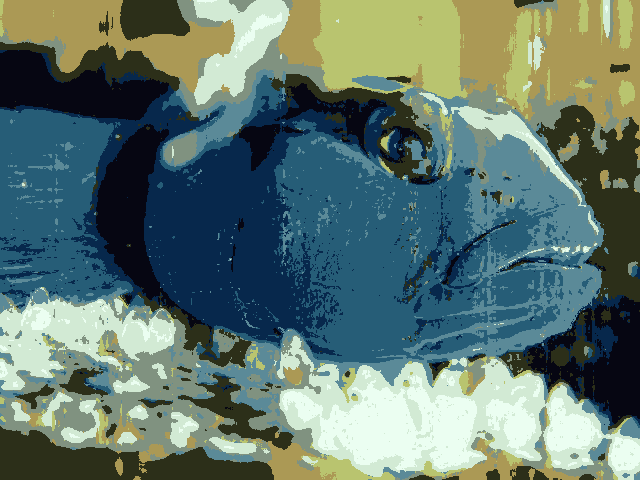
\includegraphics[width=0.7\textwidth]{parta_10_means}
\caption{10 Clusters}
\end{figure}

   
\begin{figure}[H]
\centering
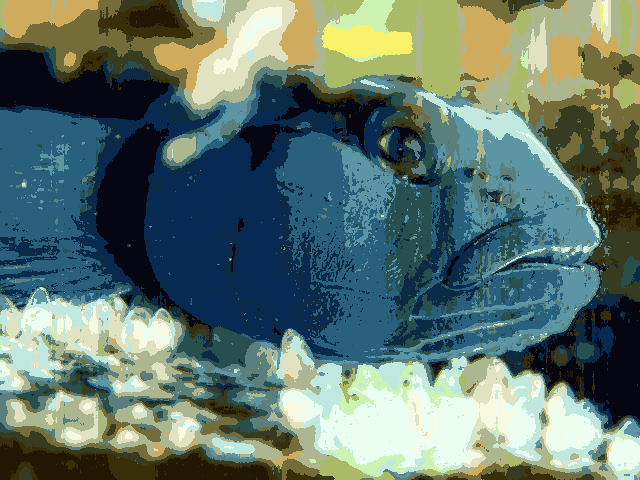
\includegraphics[width=0.7\textwidth]{parta_20_means}
\caption{20 Clusters}
\end{figure}

    
\begin{figure}[H]
\centering
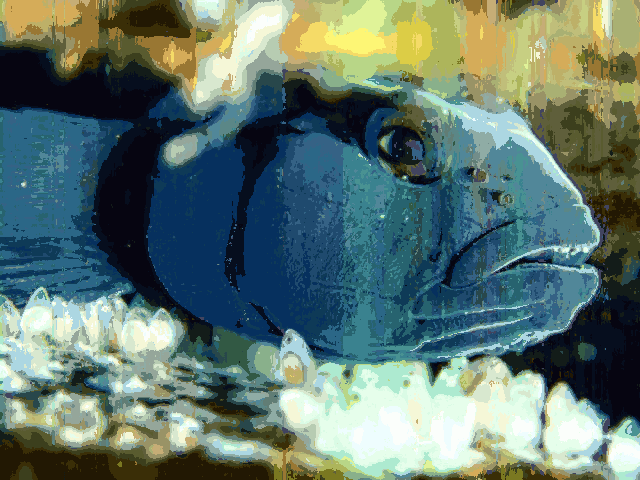
\includegraphics[width=0.7\textwidth]{parta_50_means}
\caption{50 Clusters}
\end{figure}



The code for generating the above images is as shown below.

\begin{lstlisting}
def rescale_matrix(matrix, mode="int"):
    new_matrix = matrix
    for col in range(640):
        new_matrix.loc[:, col] *= 255
    
    if mode == "int":
        new_matrix.astype(int)
    return new_matrix

def print_matrix_image(original_image, image):
    im2 = Image.new(original_image.mode, original_image.size)
    img = image.values.flatten()
    im2.putdata(img)
    im2.show()

def matricize_list(image, img_w=640, img_h=480):
    image_matrix = []
    for y in range(img_h):
        image_matrix.append(image[y*img_w:(y+1)*img_w])
    image_df = pd.DataFrame(image_matrix)
    return image_df

def rescale_weight_matrix(matrix, mode="int"):
    new_matrix = matrix
    for col in range(640):
        new_matrix.loc[:, col] *= 1000
    
    if mode == "int":
        new_matrix.astype(int)
    return new_matrix

matrix_mean_R = matricize_list(list(data["mean_R"]))
matrix_mean_G = matricize_list(list(data["mean_G"]))
matrix_mean_B = matricize_list(list(data["mean_B"]))

matrix_mean_rescaled_R = rescale_matrix(matrix_mean_R)
matrix_mean_rescaled_G = rescale_matrix(matrix_mean_G)
matrix_mean_rescaled_B = rescale_matrix(matrix_mean_B)

matrix_mean_R = matrix_mean_R.astype(int)
matrix_mean_G = matrix_mean_G.astype(int)
matrix_mean_B = matrix_mean_B.astype(int)
matrix_mean_RGB = pd.DataFrame(np.rec.fromarrays((matrix_mean_R.values, matrix_mean_G.values, matrix_mean_B.values)).tolist(),
                      columns=matrix_mean_R.columns,
                      index=matrix_mean_R.index)

print_matrix_image(working_image, matrix_mean_RGB)
\end{lstlisting}

\subsection{Part b}

We constructed the figures showing the weights linking each pixel to each cluster center. Following is the code which executes this.

\begin{lstlisting}
def print_matrix_weight(working_image, weight_image_matrix):
    im2 = Image.new("L", working_image.size)
    img = weight_image_matrix.values.flatten()
    im2.putdata(img)
    im2.show()

def weight_matrix_creation():
    for i in range(10):
        weight_image_matrix = matricize_list(list(data["weight_c"+str(i)]))
        weight_matrix_rescaled = rescale_weight_matrix(weight_image_matrix)
        print_matrix_weight(working_image, weight_matrix_rescaled)

weight_image_matrix = matricize_list(list(data["weight_c9"]))    ##c9 is for cluster 10. for cluster i, it would be c i-1
weight_matrix_rescaled = rescale_weight_matrix(weight_image_matrix)
print_matrix_weight(working_image, weight_matrix_rescaled)
\end{lstlisting}

The images generated are as shown below.

\begin{figure}[H]
\centering
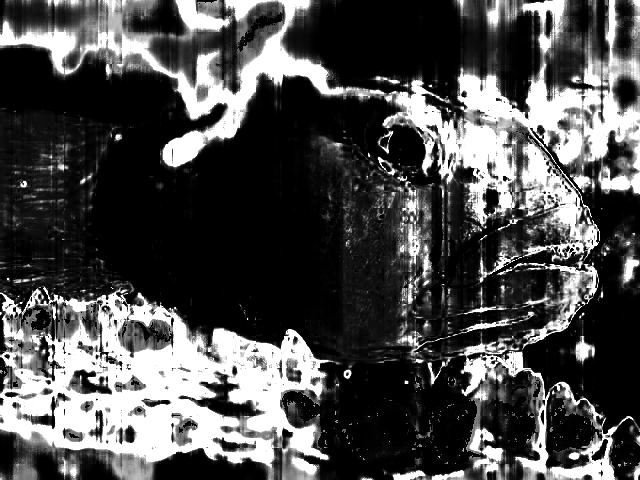
\includegraphics[width=0.7\textwidth]{partb_wts_cluster0}
\caption{Cluster 1}
\end{figure}

\begin{figure}[H]
\centering
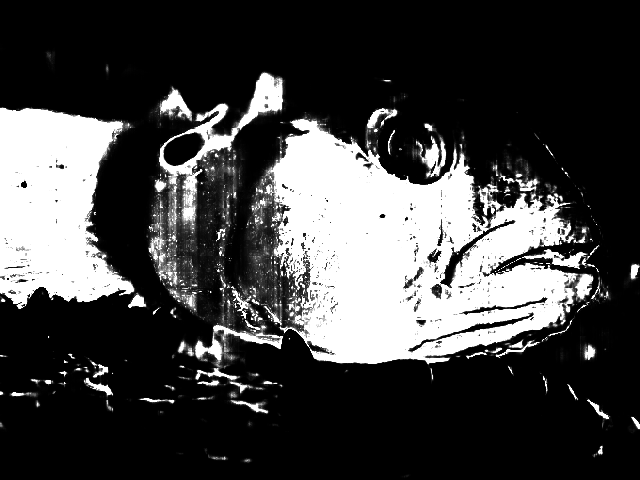
\includegraphics[width=0.7\textwidth]{partb_wts_cluster1}
\caption{Cluster 2}
\end{figure}

\begin{figure}[H]
\centering
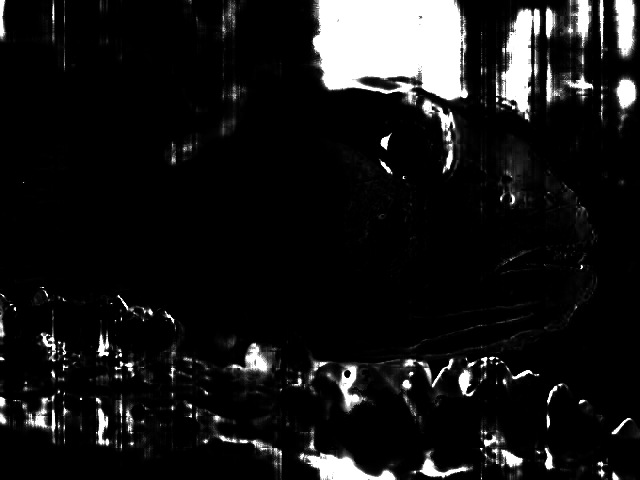
\includegraphics[width=0.7\textwidth]{partb_wts_cluster2}
\caption{Cluster 3}
\end{figure}

\begin{figure}[H]
\centering
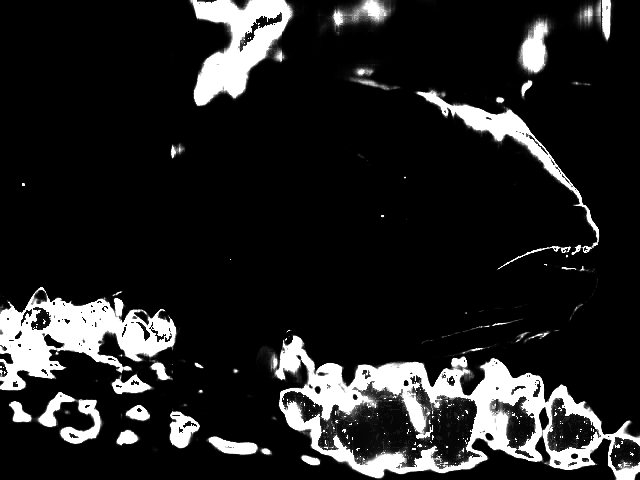
\includegraphics[width=0.7\textwidth]{partb_wts_cluster3}
\caption{Cluster 4}
\end{figure}

\begin{figure}[H]
\centering
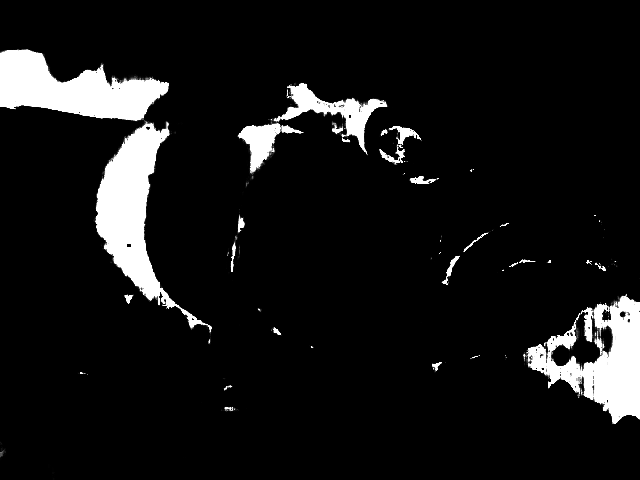
\includegraphics[width=0.7\textwidth]{partb_wts_cluster4}
\caption{Cluster 5}
\end{figure}

\begin{figure}[H]
\centering
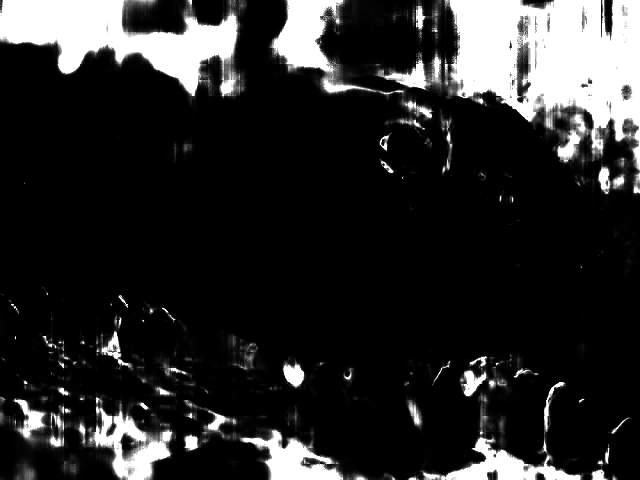
\includegraphics[width=0.7\textwidth]{partb_wts_cluster5}
\caption{Cluster 6}
\end{figure}

\begin{figure}[H]
\centering
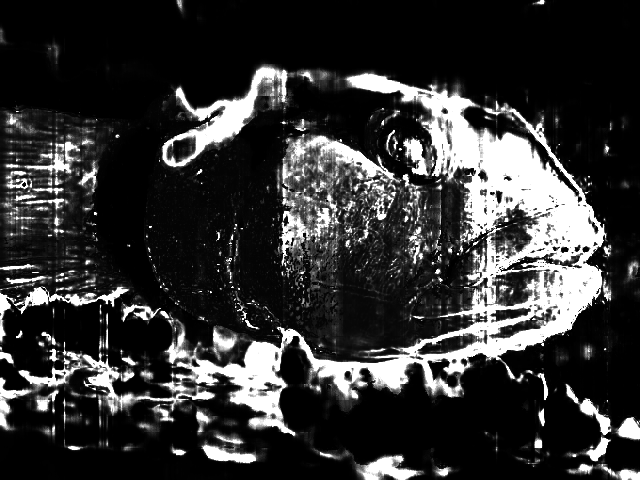
\includegraphics[width=0.7\textwidth]{partb_wts_cluster6}
\caption{Cluster 7}
\end{figure}

\begin{figure}[H]
\centering
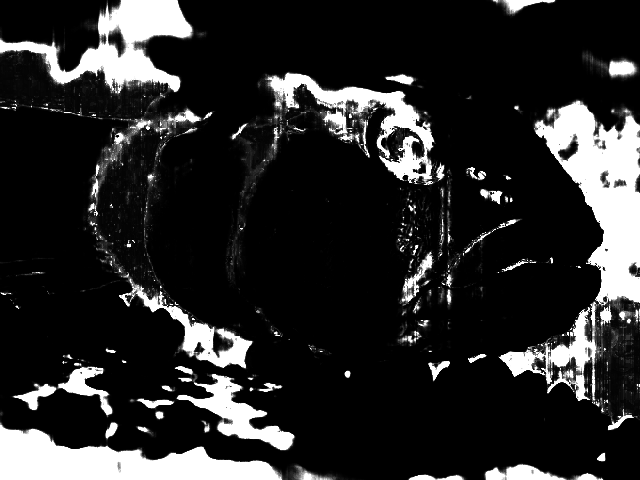
\includegraphics[width=0.7\textwidth]{partb_wts_cluster7}
\caption{Cluster 8}
\end{figure}

\begin{figure}[H]
\centering
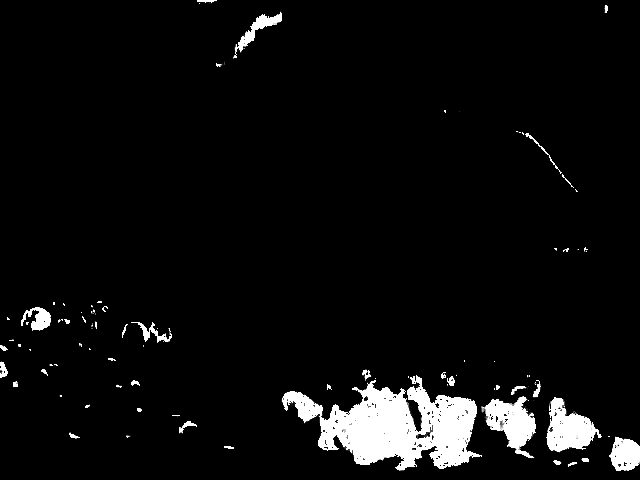
\includegraphics[width=0.7\textwidth]{partb_wts_cluster8}
\caption{Cluster 9}
\end{figure}

\begin{figure}[H]
\centering
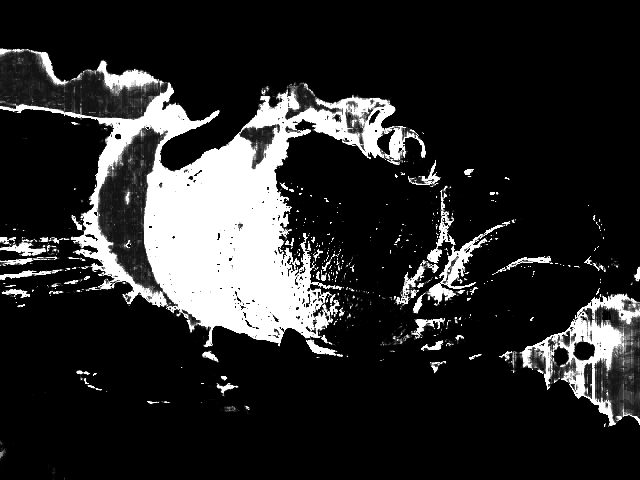
\includegraphics[width=0.7\textwidth]{partb_wts_cluster9}
\caption{Cluster 10}
\end{figure}

\subsection{Part c}

We change the covariance to \(0.1 X I\) and ran the code. 

\begin{lstlisting}
rvalues=rgb_normalized_list[0].values.flatten()
gvalues=rgb_normalized_list[1].values.flatten()
bvalues=rgb_normalized_list[2].values.flatten()
list_of_tuples = list(zip(rvalues, gvalues, bvalues))  
data=pd.DataFrame(list_of_tuples, columns = ['R', 'G', 'B'])
#Number of clusters
k=50
#Initializing the covariance matrix
cov = []
for i in range(k):
    cov.append(0.1*np.eye(data.shape[1]))
cov = np.array(cov)
means,cov,weights,b,log_likelihoods,likelihood=EM_function(data,cov,k,500)
#Plotting the log-likelihood
plt.plot(log_likelihoods)
likelihood = np.array(likelihood)
#Finding the closest cluster for each pixel
predictions = np.argmax(likelihood, axis=0)
data['cluster']=predictions
data['mean_R']=np.zeros(data.shape[0])
data['mean_G']=np.zeros(data.shape[0])
data['mean_B']=np.zeros(data.shape[0])
for i in range(data.shape[0]):
    data.at[i,'mean_R']=means[data.at[i,'cluster']][0]
    data.at[i,'mean_G']=means[data.at[i,'cluster']][1]
    data.at[i,'mean_B']=means[data.at[i,'cluster']][2]
for i in range(k):
    data['weight_c'+str(i)]=b[i]
\end{lstlisting}

We ran the code for 500 iterations. The convergence of log likelhood values for 10 clusters is as shown below. 

\begin{figure}[H]
\centering
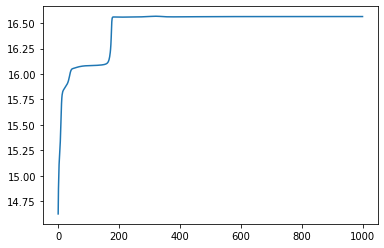
\includegraphics[width=0.7\textwidth]{Convergence_partb_10}
\end{figure}

The values converge around 200 iterations.

The following are the images obtained by replacing each pixel with the mean of its cluster center. 

\begin{figure}[H]
\centering
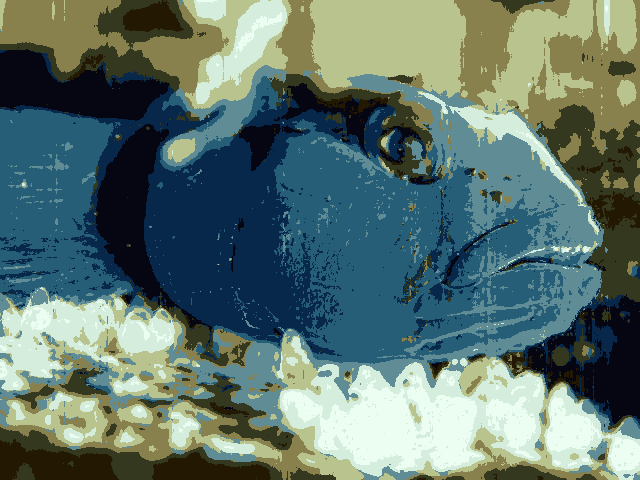
\includegraphics[width=0.7\textwidth]{partc_10_means}
\caption{10 Clusters}
\end{figure}

\begin{figure}[H]
\centering
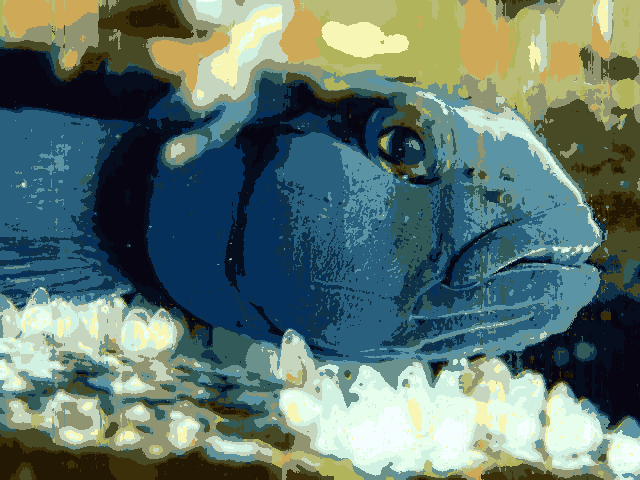
\includegraphics[width=0.7\textwidth]{partc_20_means}
\caption{20 Clusters}
\end{figure}

\begin{figure}[H]
\centering
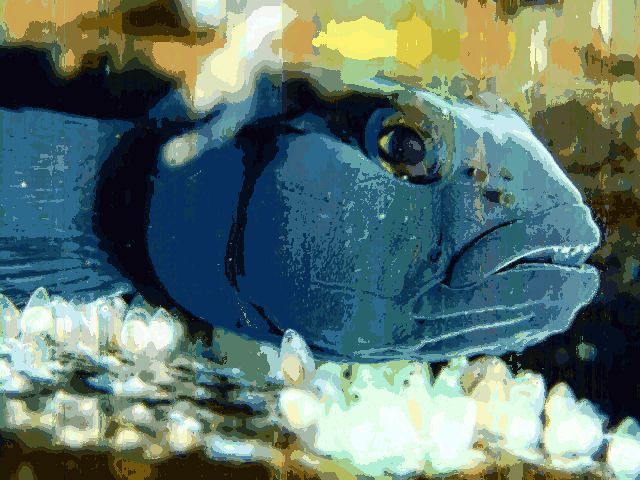
\includegraphics[width=0.7\textwidth]{partc_50_means}
\caption{50 Clusters}
\end{figure}

Following are the new set of weight maps.

\begin{figure}[H]
\centering
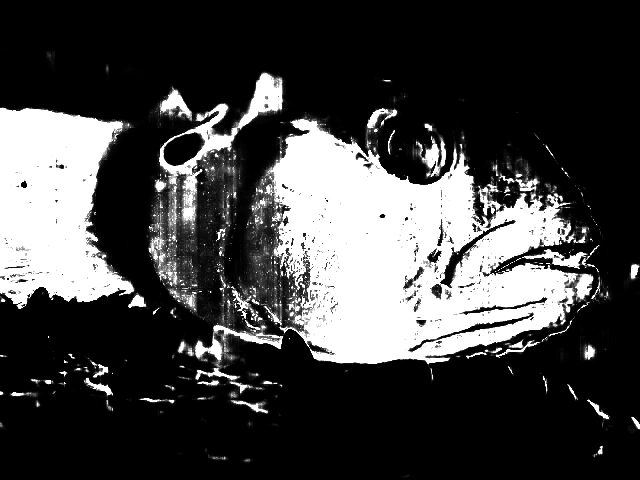
\includegraphics[width=0.7\textwidth]{partc_wts_cluster0}
\caption{Cluster 1}
\end{figure}

\begin{figure}[H]
\centering
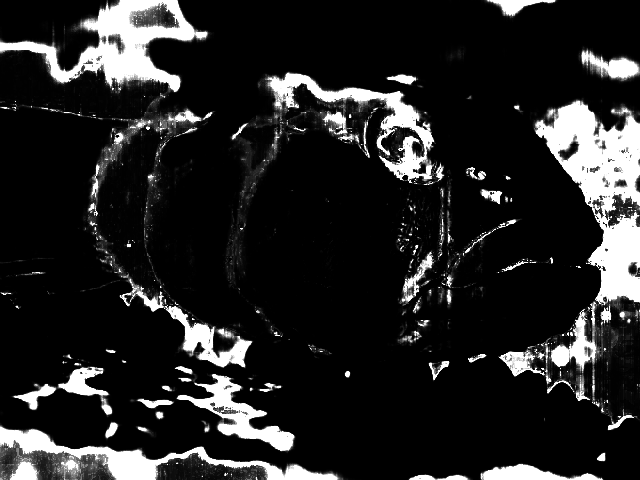
\includegraphics[width=0.7\textwidth]{partc_wts_cluster1}
\caption{Cluster 2}
\end{figure}

\begin{figure}[H]
\centering
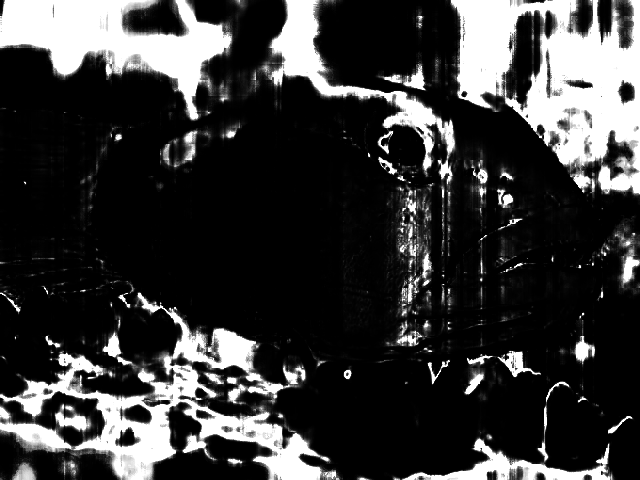
\includegraphics[width=0.7\textwidth]{partc_wts_cluster2}
\caption{Cluster 3}
\end{figure}

\begin{figure}[H]
\centering
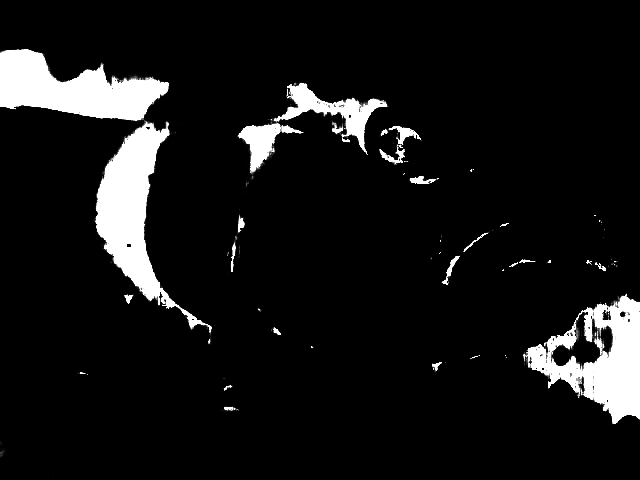
\includegraphics[width=0.7\textwidth]{partc_wts_cluster3}
\caption{Cluster 4}
\end{figure}

\begin{figure}[H]
\centering
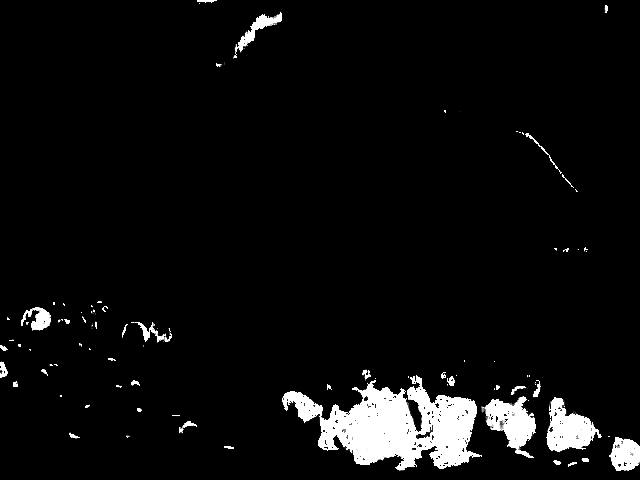
\includegraphics[width=0.7\textwidth]{partc_wts_cluster4}
\caption{Cluster 5}
\end{figure}

\begin{figure}[H]
\centering
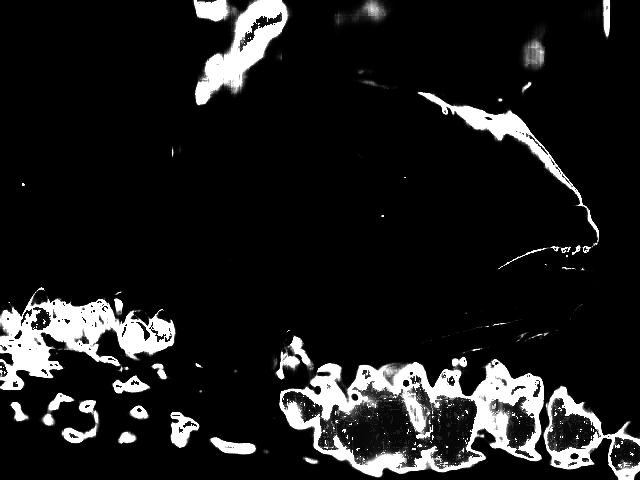
\includegraphics[width=0.7\textwidth]{partc_wts_cluster5}
\caption{Cluster 6}
\end{figure}

\begin{figure}[H]
\centering
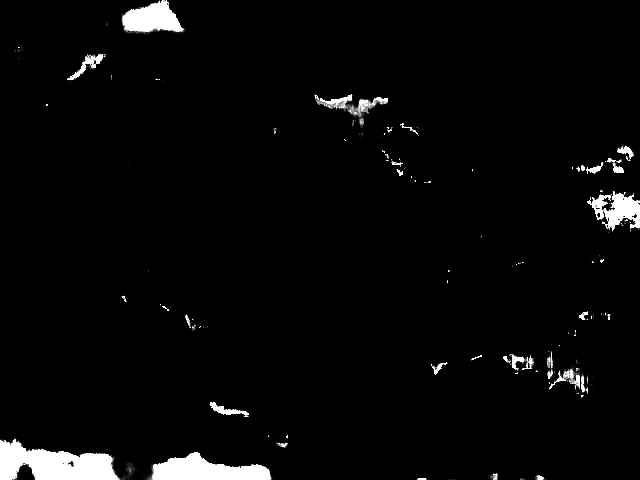
\includegraphics[width=0.7\textwidth]{partc_wts_cluster6}
\caption{Cluster 7}
\end{figure}

\begin{figure}[H]
\centering
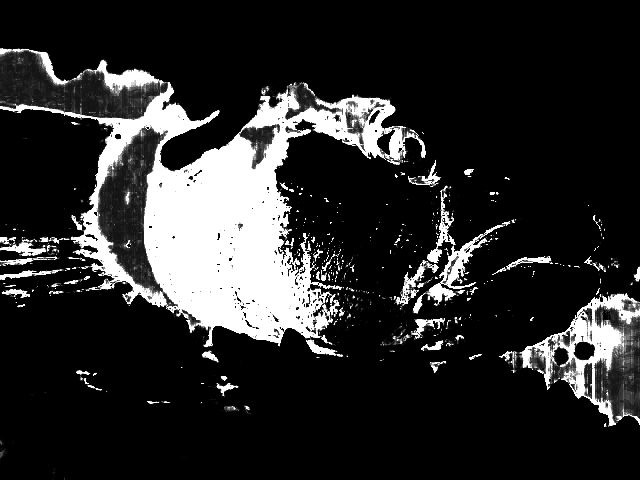
\includegraphics[width=0.7\textwidth]{partc_wts_cluster7}
\caption{Cluster 8}
\end{figure}

\begin{figure}[H]
\centering
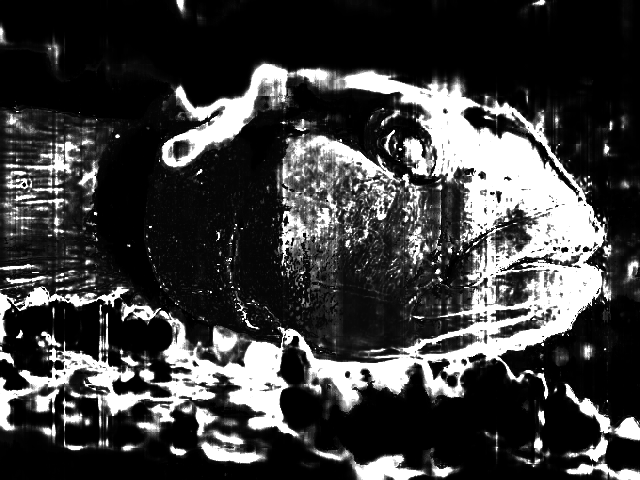
\includegraphics[width=0.7\textwidth]{partc_wts_cluster8}
\caption{Cluster 9}
\end{figure}

\begin{figure}[H]
\centering
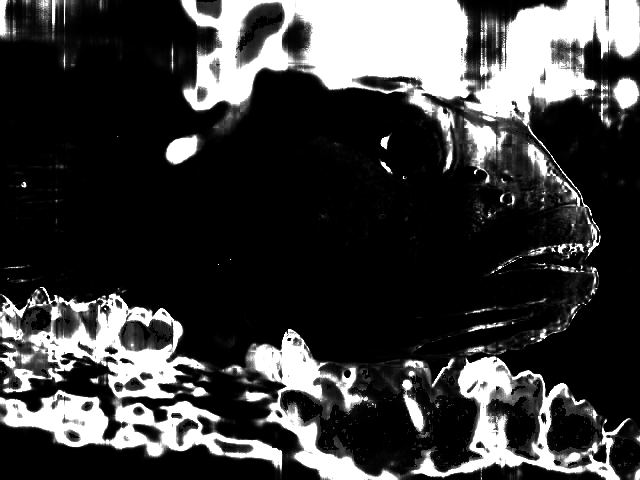
\includegraphics[width=0.7\textwidth]{partc_wts_cluster9}
\caption{Cluster 10}
\end{figure}

\subsection{Part d}

We estimated the covariance of pixel values by assuming that pixels are normally distributed and clustered them using EM. The code for this is as given below.

\begin{lstlisting}
rvalues=rgb_normalized_list[0].values.flatten()
gvalues=rgb_normalized_list[1].values.flatten()
bvalues=rgb_normalized_list[2].values.flatten()
list_of_tuples = list(zip(rvalues, gvalues, bvalues))  
data=pd.DataFrame(list_of_tuples, columns = ['R', 'G', 'B'])
#Number of clusters
k=50
#Initializing the covariance matrix
cov = []
for i in range(k):
    cov.append(np.array(data.cov()))
cov = np.array(cov)
means,cov,weights,b,log_likelihoods,likelihood=EM_function(data,cov,k,500)
#Plotting the log-likelihood
plt.plot(log_likelihoods)
likelihood = np.array(likelihood)
#Finding the closest cluster for each pixel
predictions = np.argmax(likelihood, axis=0)
data['cluster']=predictions
data['mean_R']=np.zeros(data.shape[0])
data['mean_G']=np.zeros(data.shape[0])
data['mean_B']=np.zeros(data.shape[0])
for i in range(data.shape[0]):
    data.at[i,'mean_R']=means[data.at[i,'cluster']][0]
    data.at[i,'mean_G']=means[data.at[i,'cluster']][1]
    data.at[i,'mean_B']=means[data.at[i,'cluster']][2]
for i in range(k):
    data['weight_c'+str(i)]=b[i]
\end{lstlisting}

 We ran the code for 500 iterations. The convergence of log likelhood values for 10 clusters is as shown below. 

\begin{figure}[H]
\centering
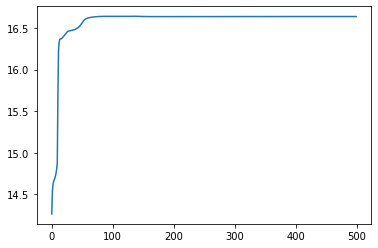
\includegraphics[width=0.7\textwidth]{Convergence_partd_10}
\end{figure}

The values converge around 100 iterations.

The following are the images obtained by replacing each pixel with the mean of its cluster center. 

\begin{figure}[H]
\centering
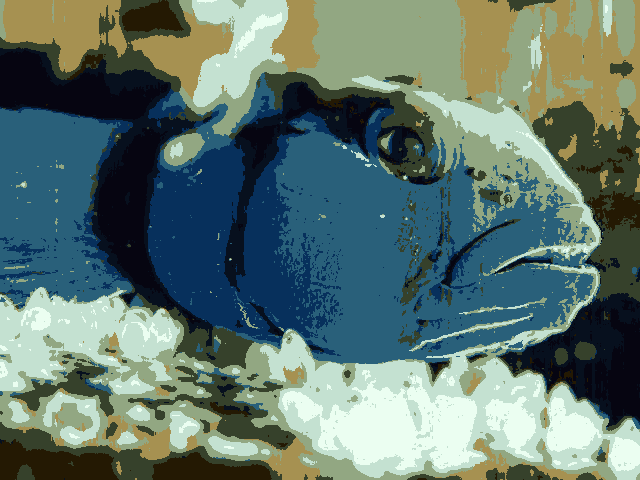
\includegraphics[width=0.7\textwidth]{partd_10_means}
\caption{10 Clusters}
\end{figure}

\begin{figure}[H]
\centering
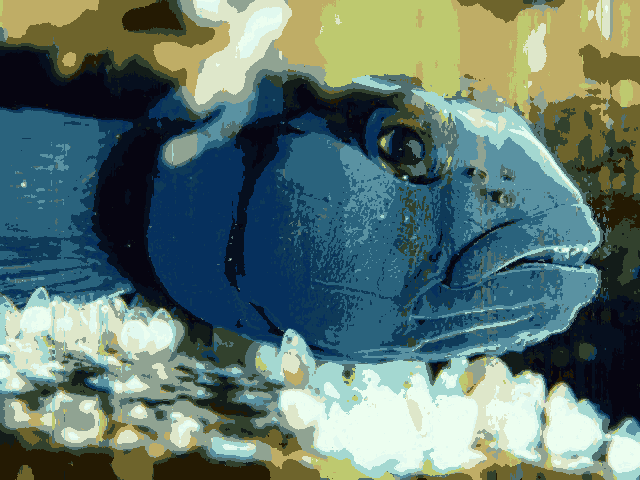
\includegraphics[width=0.7\textwidth]{partd_20_means}
\caption{20 Clusters}
\end{figure}

\begin{figure}[H]
\centering
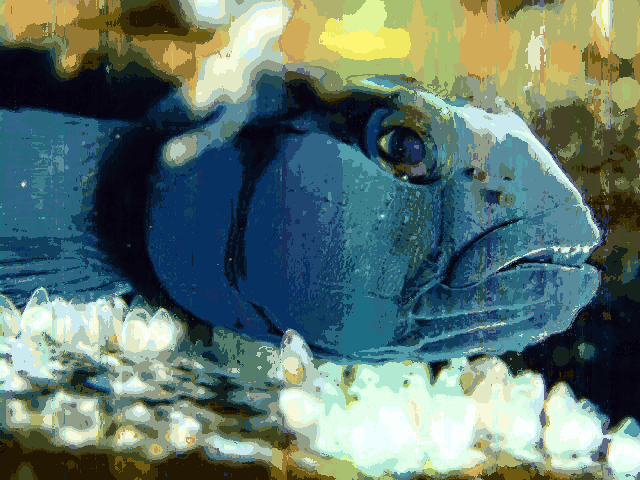
\includegraphics[width=0.7\textwidth]{partd_50_means}
\caption{50 Clusters}
\end{figure}

Following are the new set of weight maps.

\begin{figure}[H]
\centering
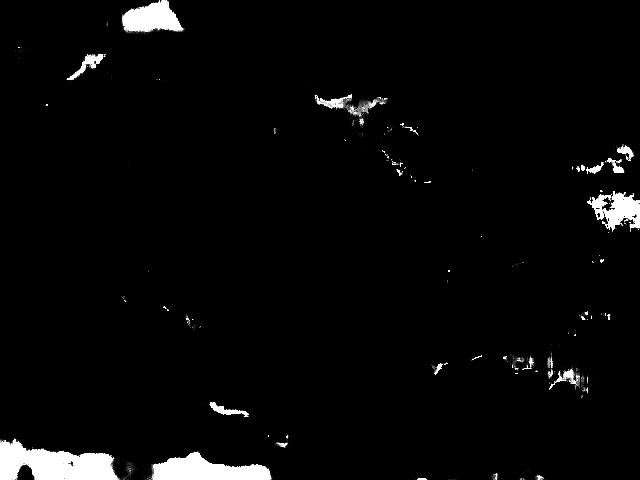
\includegraphics[width=0.7\textwidth]{partd_wts_cluster0}
\caption{Cluster 1}
\end{figure}

\begin{figure}[H]
\centering
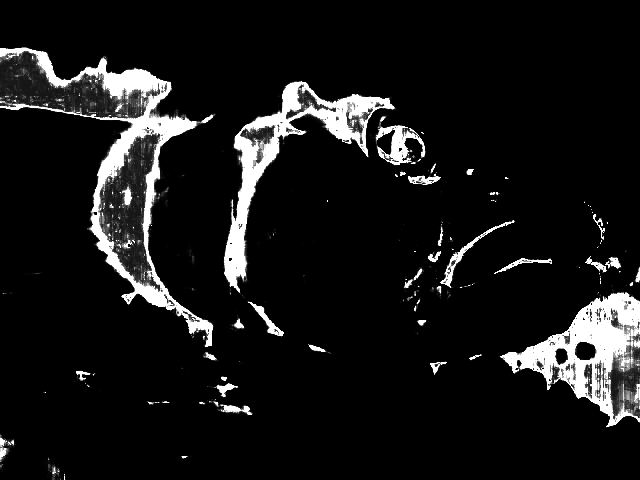
\includegraphics[width=0.7\textwidth]{partd_wts_cluster1}
\caption{Cluster 2}
\end{figure}

\begin{figure}[H]
\centering
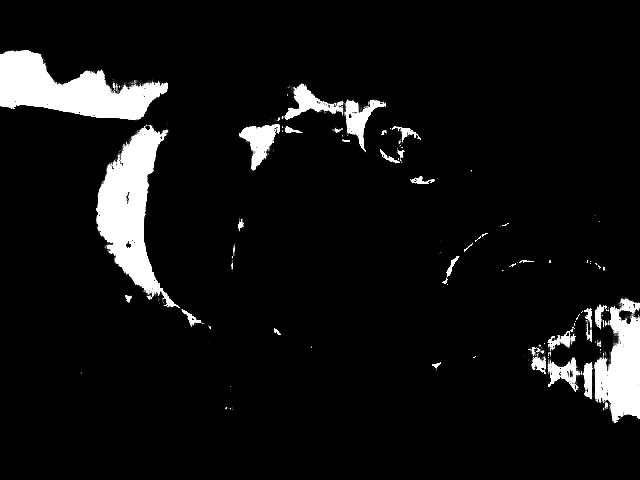
\includegraphics[width=0.7\textwidth]{partd_wts_cluster2}
\caption{Cluster 3}
\end{figure}

\begin{figure}[H]
\centering
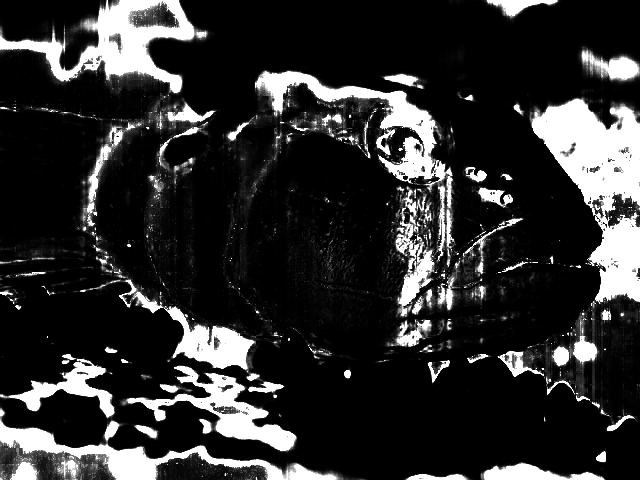
\includegraphics[width=0.7\textwidth]{partd_wts_cluster3}
\caption{Cluster 4}
\end{figure}

\begin{figure}[H]
\centering
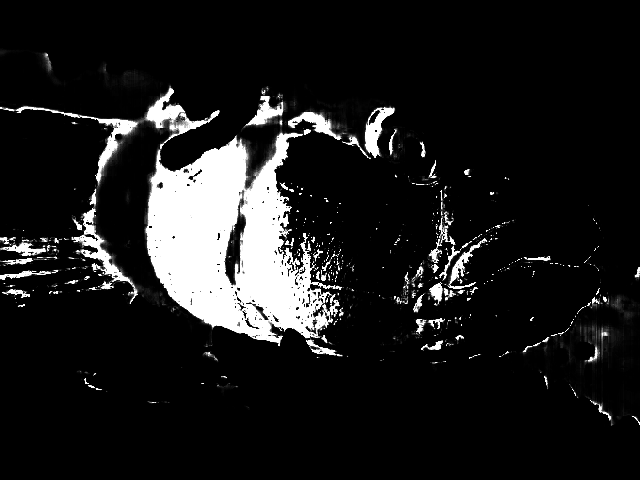
\includegraphics[width=0.7\textwidth]{partd_wts_cluster4}
\caption{Cluster 5}
\end{figure}

\begin{figure}[H]
\centering
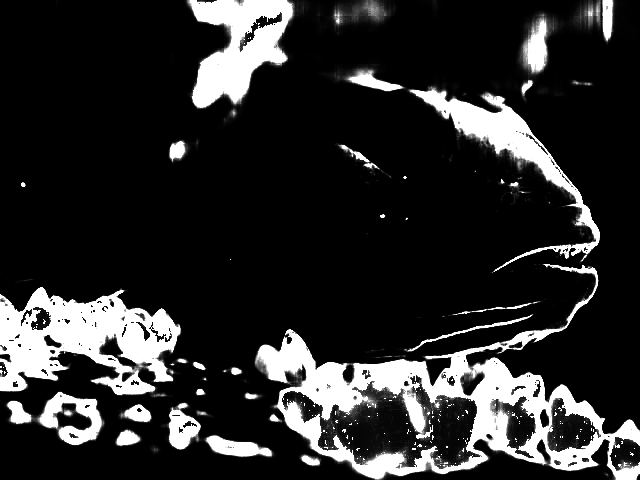
\includegraphics[width=0.7\textwidth]{partd_wts_cluster5}
\caption{Cluster 6}
\end{figure}

\begin{figure}[H]
\centering
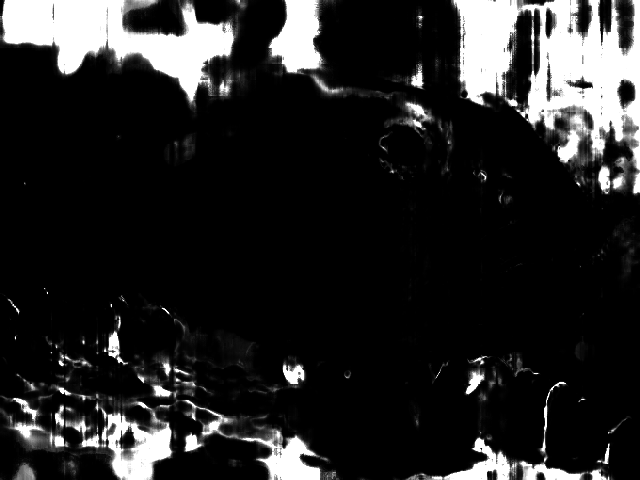
\includegraphics[width=0.7\textwidth]{partd_wts_cluster6}
\caption{Cluster 7}
\end{figure}

\begin{figure}[H]
\centering
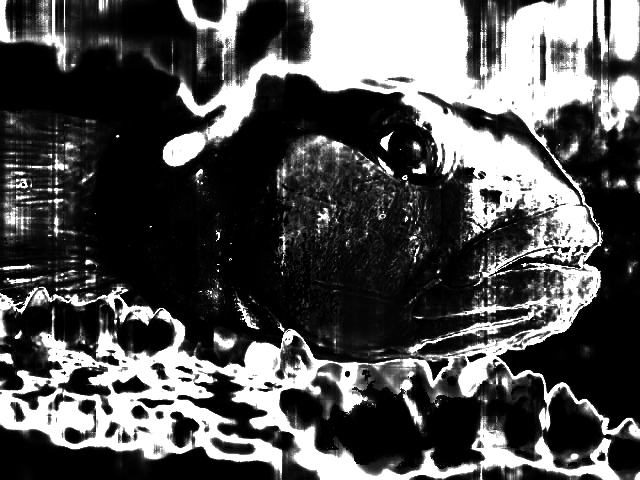
\includegraphics[width=0.7\textwidth]{partd_wts_cluster7}
\caption{Cluster 8}
\end{figure}

\begin{figure}[H]
\centering
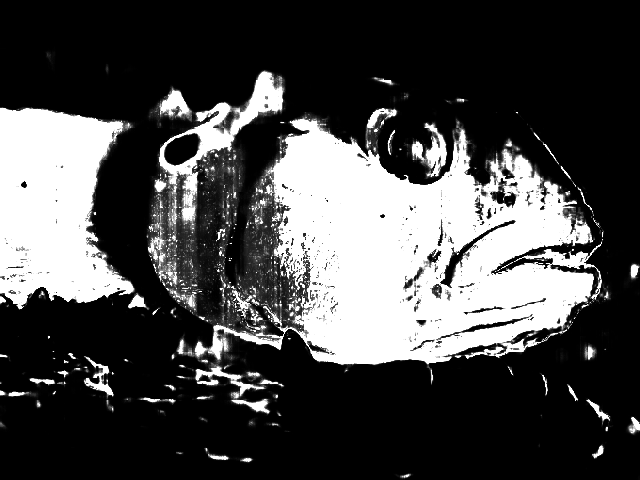
\includegraphics[width=0.7\textwidth]{partd_wts_cluster8}
\caption{Cluster 9}
\end{figure}

\begin{figure}[H]
\centering
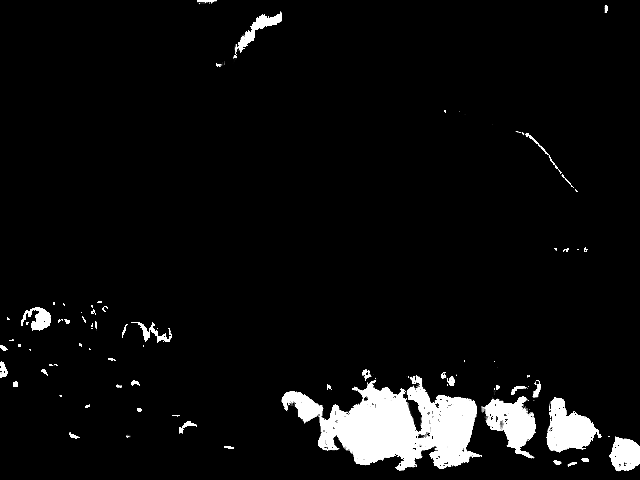
\includegraphics[width=0.7\textwidth]{partd_wts_cluster9}
\caption{Cluster 10}
\end{figure}



\end{document}